\documentclass[a4paper, 12pt]{article}

\usepackage{hyperref}
\usepackage[warn]{mathtext}
\usepackage[utf8]{inputenc}
\usepackage[T2A]{fontenc}
\usepackage[english,russian]{babel}
\usepackage{multirow}
\usepackage{amsmath,amsfonts,amssymb,amsthm,mathtools}
\usepackage{indentfirst}
\DeclareSymbolFont{T2Aletters}{T2A}{cmr}{m}{it}
\usepackage{ gensymb }
\mathtoolsset{showonlyrefs=true}
\usepackage{euscript}
\usepackage{mathrsfs}
\usepackage[left=2cm,right=2cm,top=2cm,bottom=2cm]{geometry}
\usepackage{graphicx}
\usepackage{wrapfig}
\usepackage[rgb]{xcolor}
\hypersetup{
colorlinks=true,
urlcolor=blue
}


\title{Лабораторная работа}
\author{Гисич Арсений Б03-102}
\date{2022}

\begin{document}

	\begin{center}
		{\large МОСКОВСКИЙ ФИЗИКО-ТЕХНИЧЕСКИЙ ИНСТИТУТ (НАЦИОНАЛЬНЫЙ ИССЛЕДОВАТЕЛЬСКИЙ УНИВЕРСИТЕТ)}
	\end{center}
	\vspace{5 cm}
	{\Large
		\begin{center}
			{\bf Лабораторная работа 3.6.1}\\[0.2 cm]
			Спектральный анализ электрических сигналов
		\end{center}
	}
	\vspace{4 cm}
	\begin{flushright}
		{\Large Выполнил: \\
			\vspace{0.2 cm}
			Гисич Арсений \\
			\vspace{0.2 cm}
			Б03-102 \\}
	\end{flushright}
	\vspace{9 cm}
	\begin{center}
		Долгопрудный\\[0.1 cm]
		2022
	\end{center}
\thispagestyle{empty}

\section{Аннотация}

В работе изучается спектральный состав периодических электрических сигналов различной формы: последовательности прямоугольных импульсов, последовательности цугов и амплитудно модулированных гармонических колебаний. Спектры этих сигналов наблюдаются с помощью цифрового осциллографа и сравниваются с рассчитанными теоретически. 

\section{Теоретические сведения}

Представление периодического сигнала в виде суммы гармонических сигналов называется разложением в ряд Фурье.
	
Пусть заданная функция $f(t)$ периодически повторяется с частотой $\Omega_{1}=\dfrac{2\pi}{T},$ где $T$ --- период повторения. Ее разложение в ряд Фурье имеет вид
	
$$ f(t)=\dfrac{a_{0}}{2}+ \sum\limits_{n=1}^\infty [a_{n}\cos(n \Omega_{1}t)+b_{n}\sin(n \Omega_{1} t) ]$$
	
Здесь $\dfrac{a_{0}}{2}$ --- среднее значение функции $f(t)$,
	
$$ a_{n}=\dfrac{2}{T}\int\limits_{t_{1}}^{t_{1}+T}f(t)\cos(n \Omega_{1} t)dt, $$
	
$$ b_{n}=\dfrac{2}{T}\int\limits_{t_{1}}^{t_{1}+T}f(t)\sin(n \Omega_{1} t)dt. $$
	
Рассмотрим периодические функции, которые исследуются в нашей работе.
		
\textbf{Периодическая последовательность прямоугольных импульсов} (рис.~\ref{ris1}) с амплитудой $V_{0}$, длительностью $\tau$, частотой повторения $\Omega_{1}=\dfrac{2\pi}{T},$ где $T$ --- период повторения импульсов. Найдем коэффициенты разложения ряда Фурье:
	
$$\dfrac{a_{0}}{2}=V_{0}\dfrac{\tau}{T},$$
	
$$a_{n}=\dfrac{2}{T}\int\limits_{-\frac{\tau}{2}}^{\frac{\tau}{2}}V_{0}\cos(n \Omega_{1} t)dt=2V_{0}\dfrac{\tau}{T}\dfrac{\sin(n \Omega_{1} \frac{\tau}{2})}{n\Omega_{1}\frac{\tau}{2}} \sim \dfrac{\sin x}{x}.$$
	
Поскольку наша функция четная, все коэффициенты синусоидальных гармоник $b_{n}=0$. Спектр $a_{n}$ последовательности прямоугольных импульсов представлен на рис.~\ref{ris2} (изображен случай, когда $T$ кратно $\tau$).
		
		
\begin{figure}[h]
	\begin{minipage}[h]{0.5\linewidth}
		\center{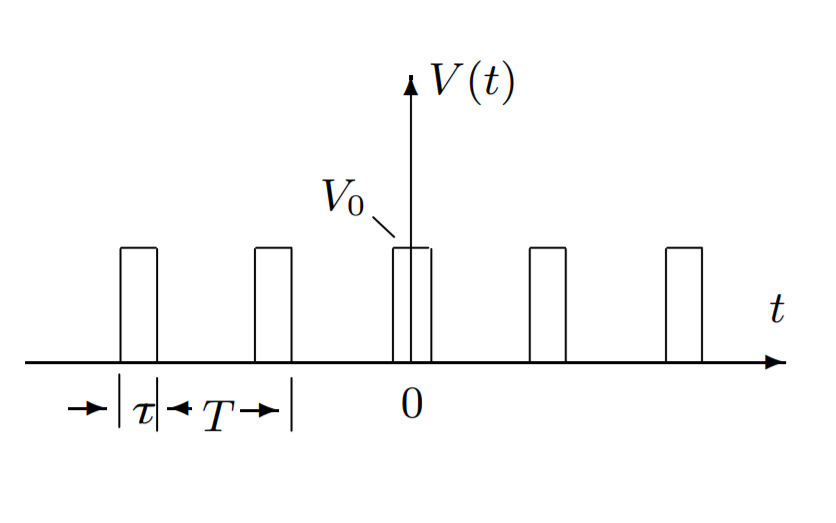
\includegraphics[width=0.9\linewidth]{sp1.png}}
		\caption{Прямоугольные импульсы}
		\label{ris1}
	\end{minipage}
	\begin{minipage}[h]{0.5\linewidth}
		\center{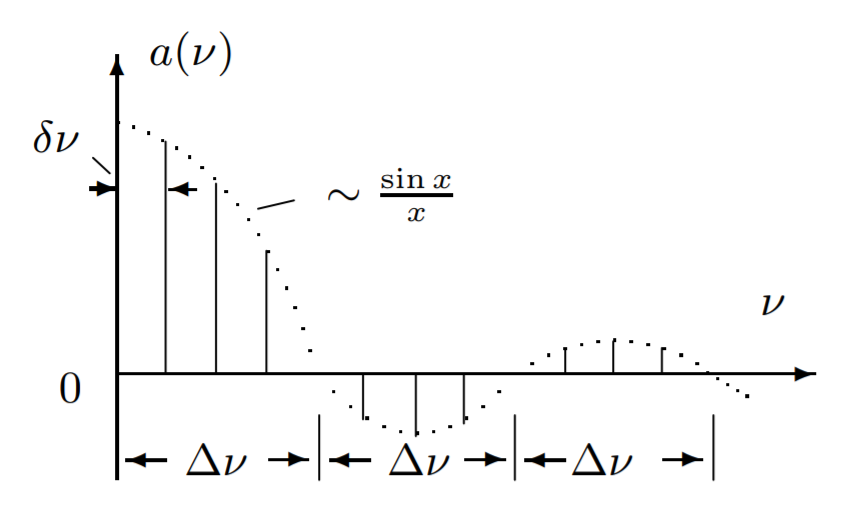
\includegraphics[width=0.9\linewidth]{sp2.png}}
		\caption{Спектр последовательности прямоугольных импульсов}
		\label{ris2}
	\end{minipage}
\end{figure}
	
Назовем \textit{шириной спектра} $\Delta \omega$ расстояние от главного максимума ($\omega =0$) до первого нуля огибающей, возникающего при $n=\dfrac{2\pi}{\tau \Omega_{1}}$. При этом 

$$\Delta \omega \tau \backsimeq 2 \pi $$

или 
	
\begin{equation}\label{neopr}
	\Delta \nu \Delta t \backsimeq 1
\end{equation}
		
Полученное соотношение взаимной связи интервалов $\Delta \nu$ и $\Delta t$ является частным случаем соотношения неопределенности в квантовой механике.
	
\textbf{Периодическая последовательность цугов} гармонического колебания $V_{0}\cos(\omega_{0}t)$ с длительностью цуга $\tau$ и периодом повторения $T$ (рис.~\ref{ris3}).
	
Функция $f(t)$ снова является четной относительно $t=0$. Коэффициент при $n$-й гармонике равен
	
$$a_{n}=\dfrac{2}{T}\int\limits_{-\frac{\tau}{2}}^{\frac{\tau}{2}}V_{0}\cos(\omega_{0}t)\cos(n \Omega_{1} t)dt=V_{0}\dfrac{\tau}{T} \bigg(\dfrac{\sin[(\omega_{0}-n\Omega_{1})\frac{\tau}{2}]}{(\omega_{0}-n\Omega_{1})\frac{\tau}{2}}+\dfrac{\sin[(\omega_{0}+n\Omega_{1})\frac{\tau}{2}]}{(\omega_{0}+n\Omega_{1})\frac{\tau}{2}} \bigg)$$ 
	
Зависимость для случая, когда $\frac{T}{\tau}$ равно целому числу, представлена на рис.~\ref{ris4}. Сравнивая спектр последовательности прямоугольных импульсов и цугов мы видим, что они аналогичны, но их максимумы сдвинуты по частоте на величину $\omega_{0}$.
	
\begin{figure}[h]
	\begin{minipage}[h]{0.5\linewidth}
		\center{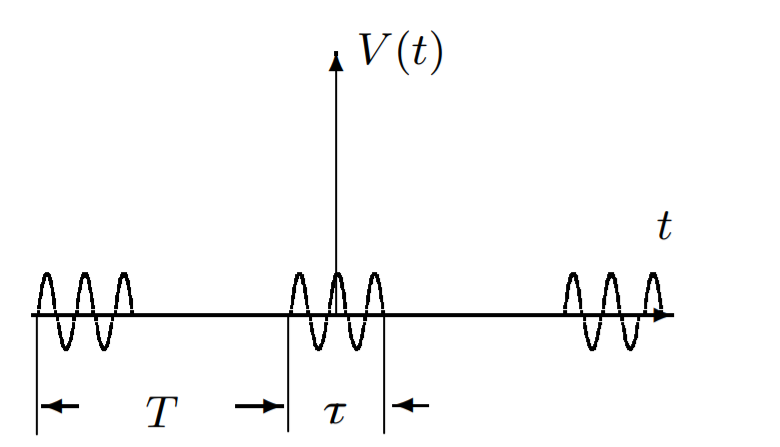
\includegraphics[width=0.9\linewidth]{sp3.png}}
		\caption{Последовательность цугов}
		\label{ris3}
	\end{minipage}
	\begin{minipage}[h]{0.5\linewidth}
		\center{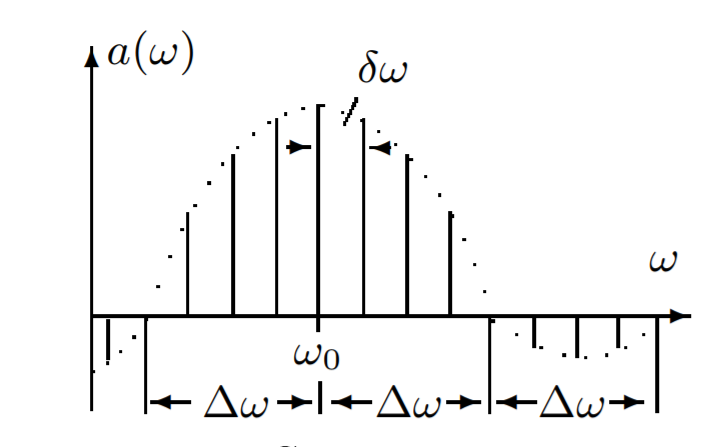
\includegraphics[width=0.9\linewidth]{sp4.png}}
		\caption{Спектр последовательности цугов}
		\label{ris4}
	\end{minipage}
\end{figure}

\textbf{Амплитудно-модулированные колебания.} Рассмотрим гармонические колебания высокой частоты $\omega_{0}$ , амплитуда которых медленно меняется по гармоническому закону с частотой $\Omega$ ($\Omega \ll \omega_{0}$) (рис.~\ref{ris5}):
	
$$f(t)=A_{0}[1+m\cos\Omega t]\cos \omega_{0}t.$$
	
Коэффициент $m$ называют \textbf{глубиной модуляции}. При $m<1$ амплитуда колебаний меняется от минимальной $A_{min}=A_{0}(1-m)$ до максимальной $A_{max}=A_{0}(1+m).$ Глубина модуляции может быть представлена в виде
	
\begin{equation}\label{m}
	 m=\dfrac{A_{max}-A_{min}}{A_{max}+A_{min}}
\end{equation}
	
Простым тригонометрическим преобразованием можно найти спектр амплитудно-модулированных колебаний:

\begin{equation}\label{a}
	f(t)=A_{0}\cos(\omega_{0} t)+\dfrac{A_{0}m}{2}\cos(\omega_{0}+\Omega)t+\dfrac{A_{0}m}{2}\cos(\omega_{0}-\Omega)t.
\end{equation}
		
\begin{figure}[h]
	\begin{minipage}[h]{0.5\linewidth}
		\center{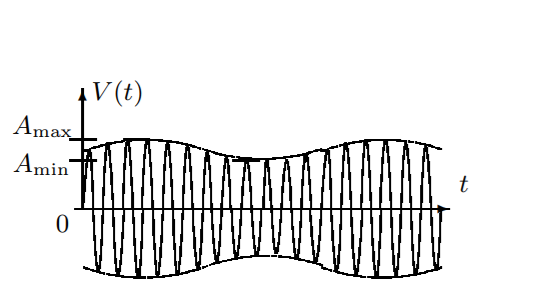
\includegraphics[width=0.9\linewidth]{sp5.png}}
		\caption{Модулированные гармонические колебания}
		\label{ris5}
	\end{minipage}
	\begin{minipage}[h]{0.5\linewidth}
		\center{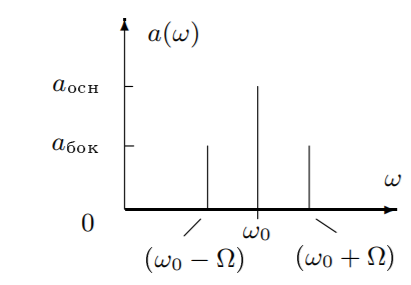
\includegraphics[width=0.9\linewidth]{sp6.png}}
		\caption{Спектр модулированных гармонических колебаний}
		\label{ris6}
	\end{minipage}
\end{figure}
		
Спектр таких колебаний содержит три составляющих: основную компоненту и две боковых (рис.~\ref{ris6}). Первое слагаемое в правой части представляет собой исходное немодулированное колебание с основной (несущей) частотой $\omega_{0}$ и амплитудой $a_{осн} = A_{0}$ . Второе и третье слагаемые соответствуют новым гармоническим колебаниям с частотами $\omega_{0} + \Omega$ и $\omega_{0} - \Omega$. Амплитуды этих двух колебаний одинаковы и составляют $\dfrac{m}{2}$ от амплитуды немодулированного колебания:
$a_{бок} = \dfrac{A_{0}m}{2}$. Начальные фазы всех трех колебаний одинаковы.

\section{Методика измерений}

Экспериментальная установка состоит из цифрового генератора сигнала и цифрового осциллографа (рис.~\ref{A}), соединённых между собой.
					
\begin{figure}[h!]
	\centering
	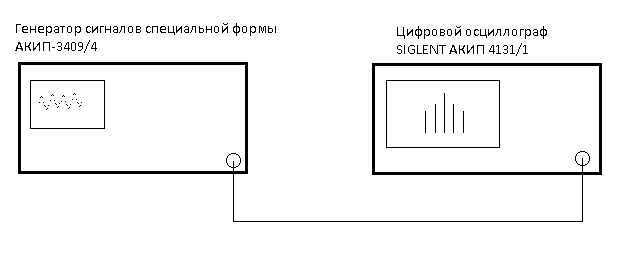
\includegraphics[width=0.8\linewidth]{sp7.png}
	\caption{Cхема для исследования спектра сигналов}
	\label{A}
\end{figure}

\section{Используемое оборудование}

\begin{enumerate}
    \item генератор сигналов произвольной формы;
    \item цифровой осциллограф;
\end{enumerate}

\section{Результаты измерений и обработка данных}

\subsection{Исследование спектра периодической последовательности прямоугольных импульсов}

Спектры сигналов при различных $\nu_{повт}$ и $\tau$ представлены на рис.~\ref{ris7}-\ref{ris14}.

При фиксированных $\nu_{повт} = 1~кГц$ и $\tau = 150~мкс$ были измерены амплитуды $a_n$ и частоты $\nu_n$ для первых 6 гармоник спектра. Рассчитанные и измеренные значения представлены в таб.~\ref{tab1}. Для сравнения теоретически рассчитанной и измеренной амплитуд сделана нормировка по наименьшему значению.

\begin{table}[h!]
\begin{center}
\begin{tabular}{|c|c|c|c|c|c|c|c|c|}
\hline
$n$ & $\nu_{т}, кГц$ & $a_{т}$ & $норм(a_{т})$ & $\nu_{изм}, кГц$ & $\delta_{\nu_{изм}}, кГц$ & $a_{изм}, мВ$ & $\delta_{a_{изм}}, мВ$ & $норм(a_{изм})$ \\ \hline
1 & 1 & 144,51 & 8,81 & 1,00 & 0,02 & 820 & 2 & 8,54 \\ \hline
2 & 2 & 128,76 & 7,85 & 2,00 & 0,02 & 736 & 2 & 7,67 \\ \hline
3 & 3 & 104,80 & 6,39 & 3,00 & 0,02 & 600 & 2 & 6,25 \\ \hline
4 & 4 & 75,68 & 4,62 & 4,00 & 0,02 & 432 & 2 & 4,50 \\ \hline
5 & 5 & 45,02 & 2,75 & 5,00 & 0,02 & 264 & 2 & 2,75 \\ \hline
6 & 6 & 16,39 & 1 & 6,00 & 0,02 & 96 & 2 & 1 \\ \hline
\end{tabular}
\end{center}
\caption{Результаты теоретического расчёта и измерений амплитуд и частот первых 6 гармоник спектра}
\label{tab1}
\end{table}

Результаты измерений зависимости ширины спектра $\Delta{\nu}$ от времени импульса $\tau$ в диапазоне от 20 до 200 мкс при фиксированной $\nu_{повт} = 1~кГц$ представлены в таб.~\ref{tab2}.

\begin{table}[h!]
\begin{center}
\begin{tabular}{|c|c|c|c|}
\hline
$\tau, мкс$ & $1/\tau, 1/c$ & $\Delta{\nu}, кГц$ & $\delta_{\Delta{\nu}}, кГц$ \\ \hline
20 & 50000 & 50,20 & 0,02 \\ \hline
70 & 14286 & 14,00 & 0,02 \\ \hline
120 & 8333 & 8,00 & 0,02 \\ \hline
170 & 5882 & 6,00 & 0,02 \\ \hline
200 & 5000 & 5,00 & 0,02 \\ \hline
\end{tabular}
\end{center}
\caption{Результаты измерений зависимости ширины спектра $\Delta{\nu}$ от длительности импульса $\tau$}
\label{tab2}
\end{table}

График зависимости $\Delta{\nu}(1/\tau)$ представлен на рис.~\ref{plot1}.

\begin{figure}[h!]
\begin{flushleft}
    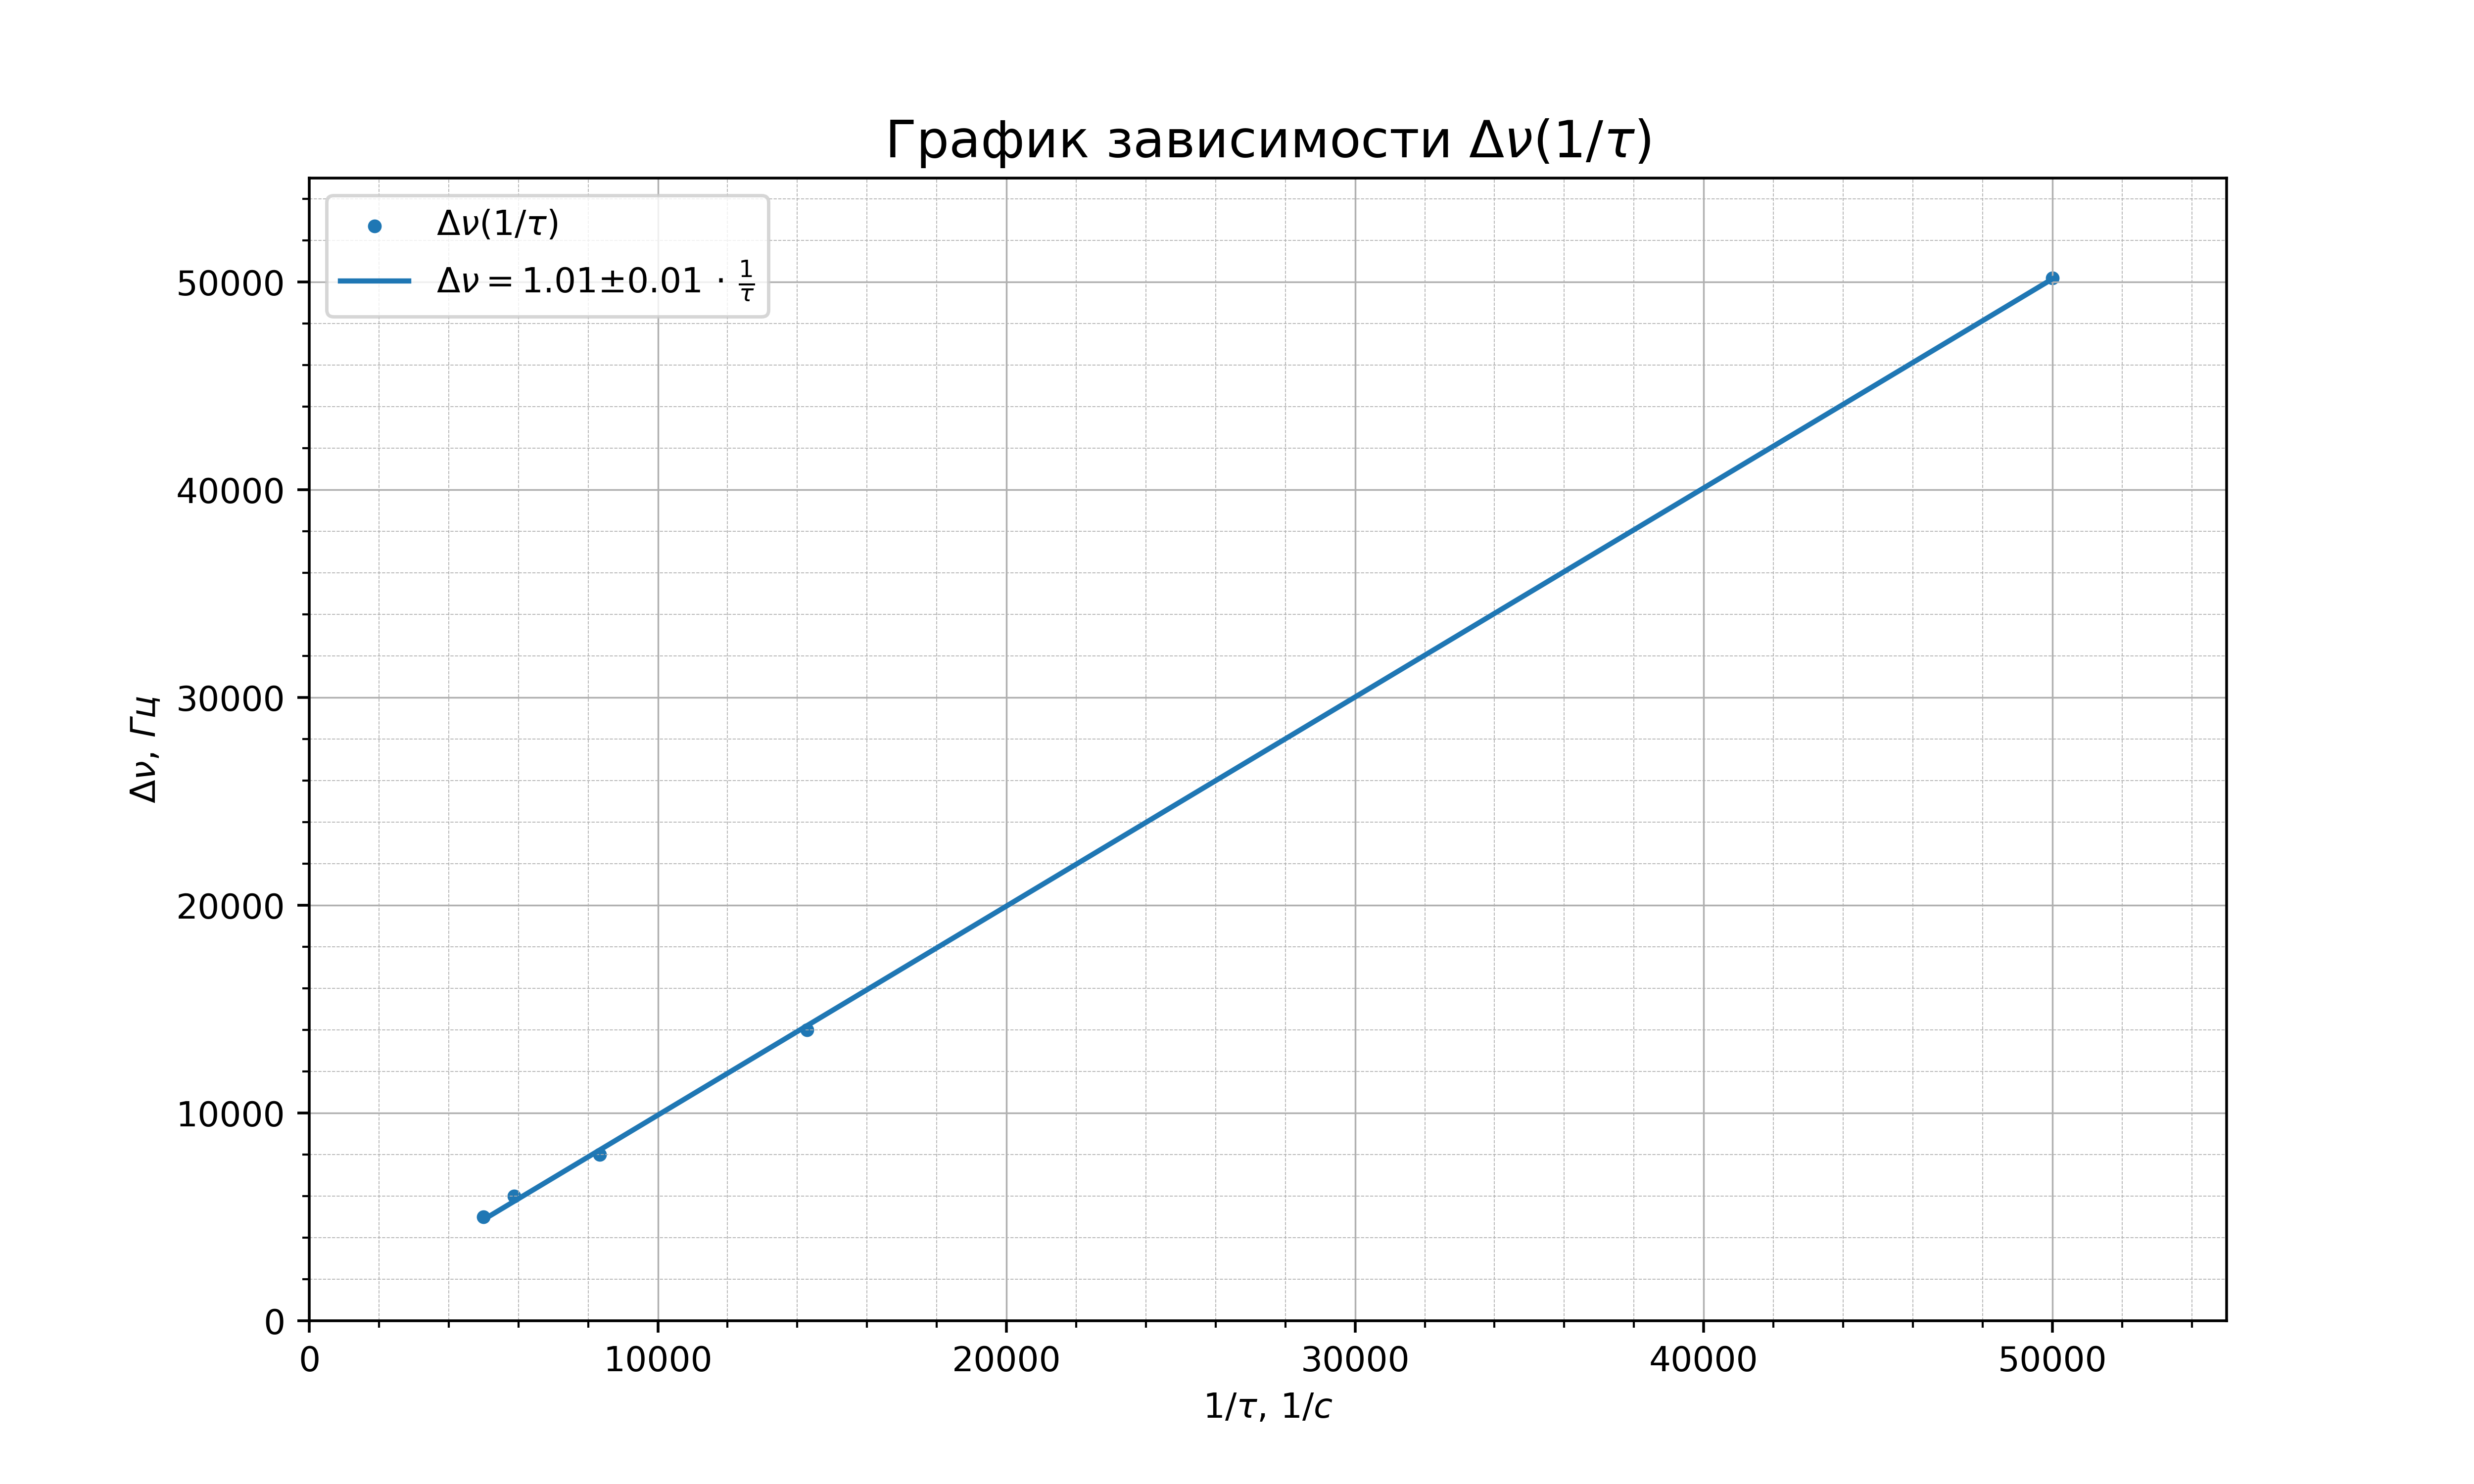
\includegraphics[scale=0.7]{3.6.1_1.png}
\end{flushleft}
\caption{График зависимости ширины спектра $\Delta{\nu}$ от обратной величины длительности импульса $1/\tau$}
\label{plot1}
\end{figure}

\newpage

\subsection{Исследование спектра периодической последовательности цугов}

Спектры сигналов при различных $\nu_0$, $T$ и $N$ представлены на рис.~\ref{ris15}-\ref{ris19}.

При фиксированных параметрах $\nu_0 = 50~кГц$ и $N = 5$ была измерена зависимость расстояния $\delta{\nu}$ между соседними спектральными компонентами сигнала от периода $T$ повторения импульсов в диапазоне $T = 0,2 - 5~мс$. Измеренные значения представлены в таб.~\ref{tab3}.

\begin{table}[h!]
\begin{center}
\begin{tabular}{|c|c|c|}
\hline
$T, мс$ & $\delta{\nu}, Гц$ & $\delta_{\delta{\nu}}, Гц$ \\ \hline
0,2 & 10000 & 10 \\ \hline
1,2 & 800 & 10 \\ \hline
2,2 & 440 & 10 \\ \hline
3,2 & 300 & 10 \\ \hline
4,2 & 240 & 10 \\ \hline
5 & 200 & 10 \\ \hline
\end{tabular}
\end{center}
\caption{Результаты измерений зависимости $\delta{\nu}(T)$}
\label{tab3}
\end{table}

Значение $\delta{\nu}$ при $T = 0,2~мс$ существенно отличается от общей зависимости и является ошибкой. Полученный график зависимости $\delta{\nu}(1/T)$ представлен на рис.~\ref{plot2}.

\begin{figure}[h!]
\begin{flushleft}
    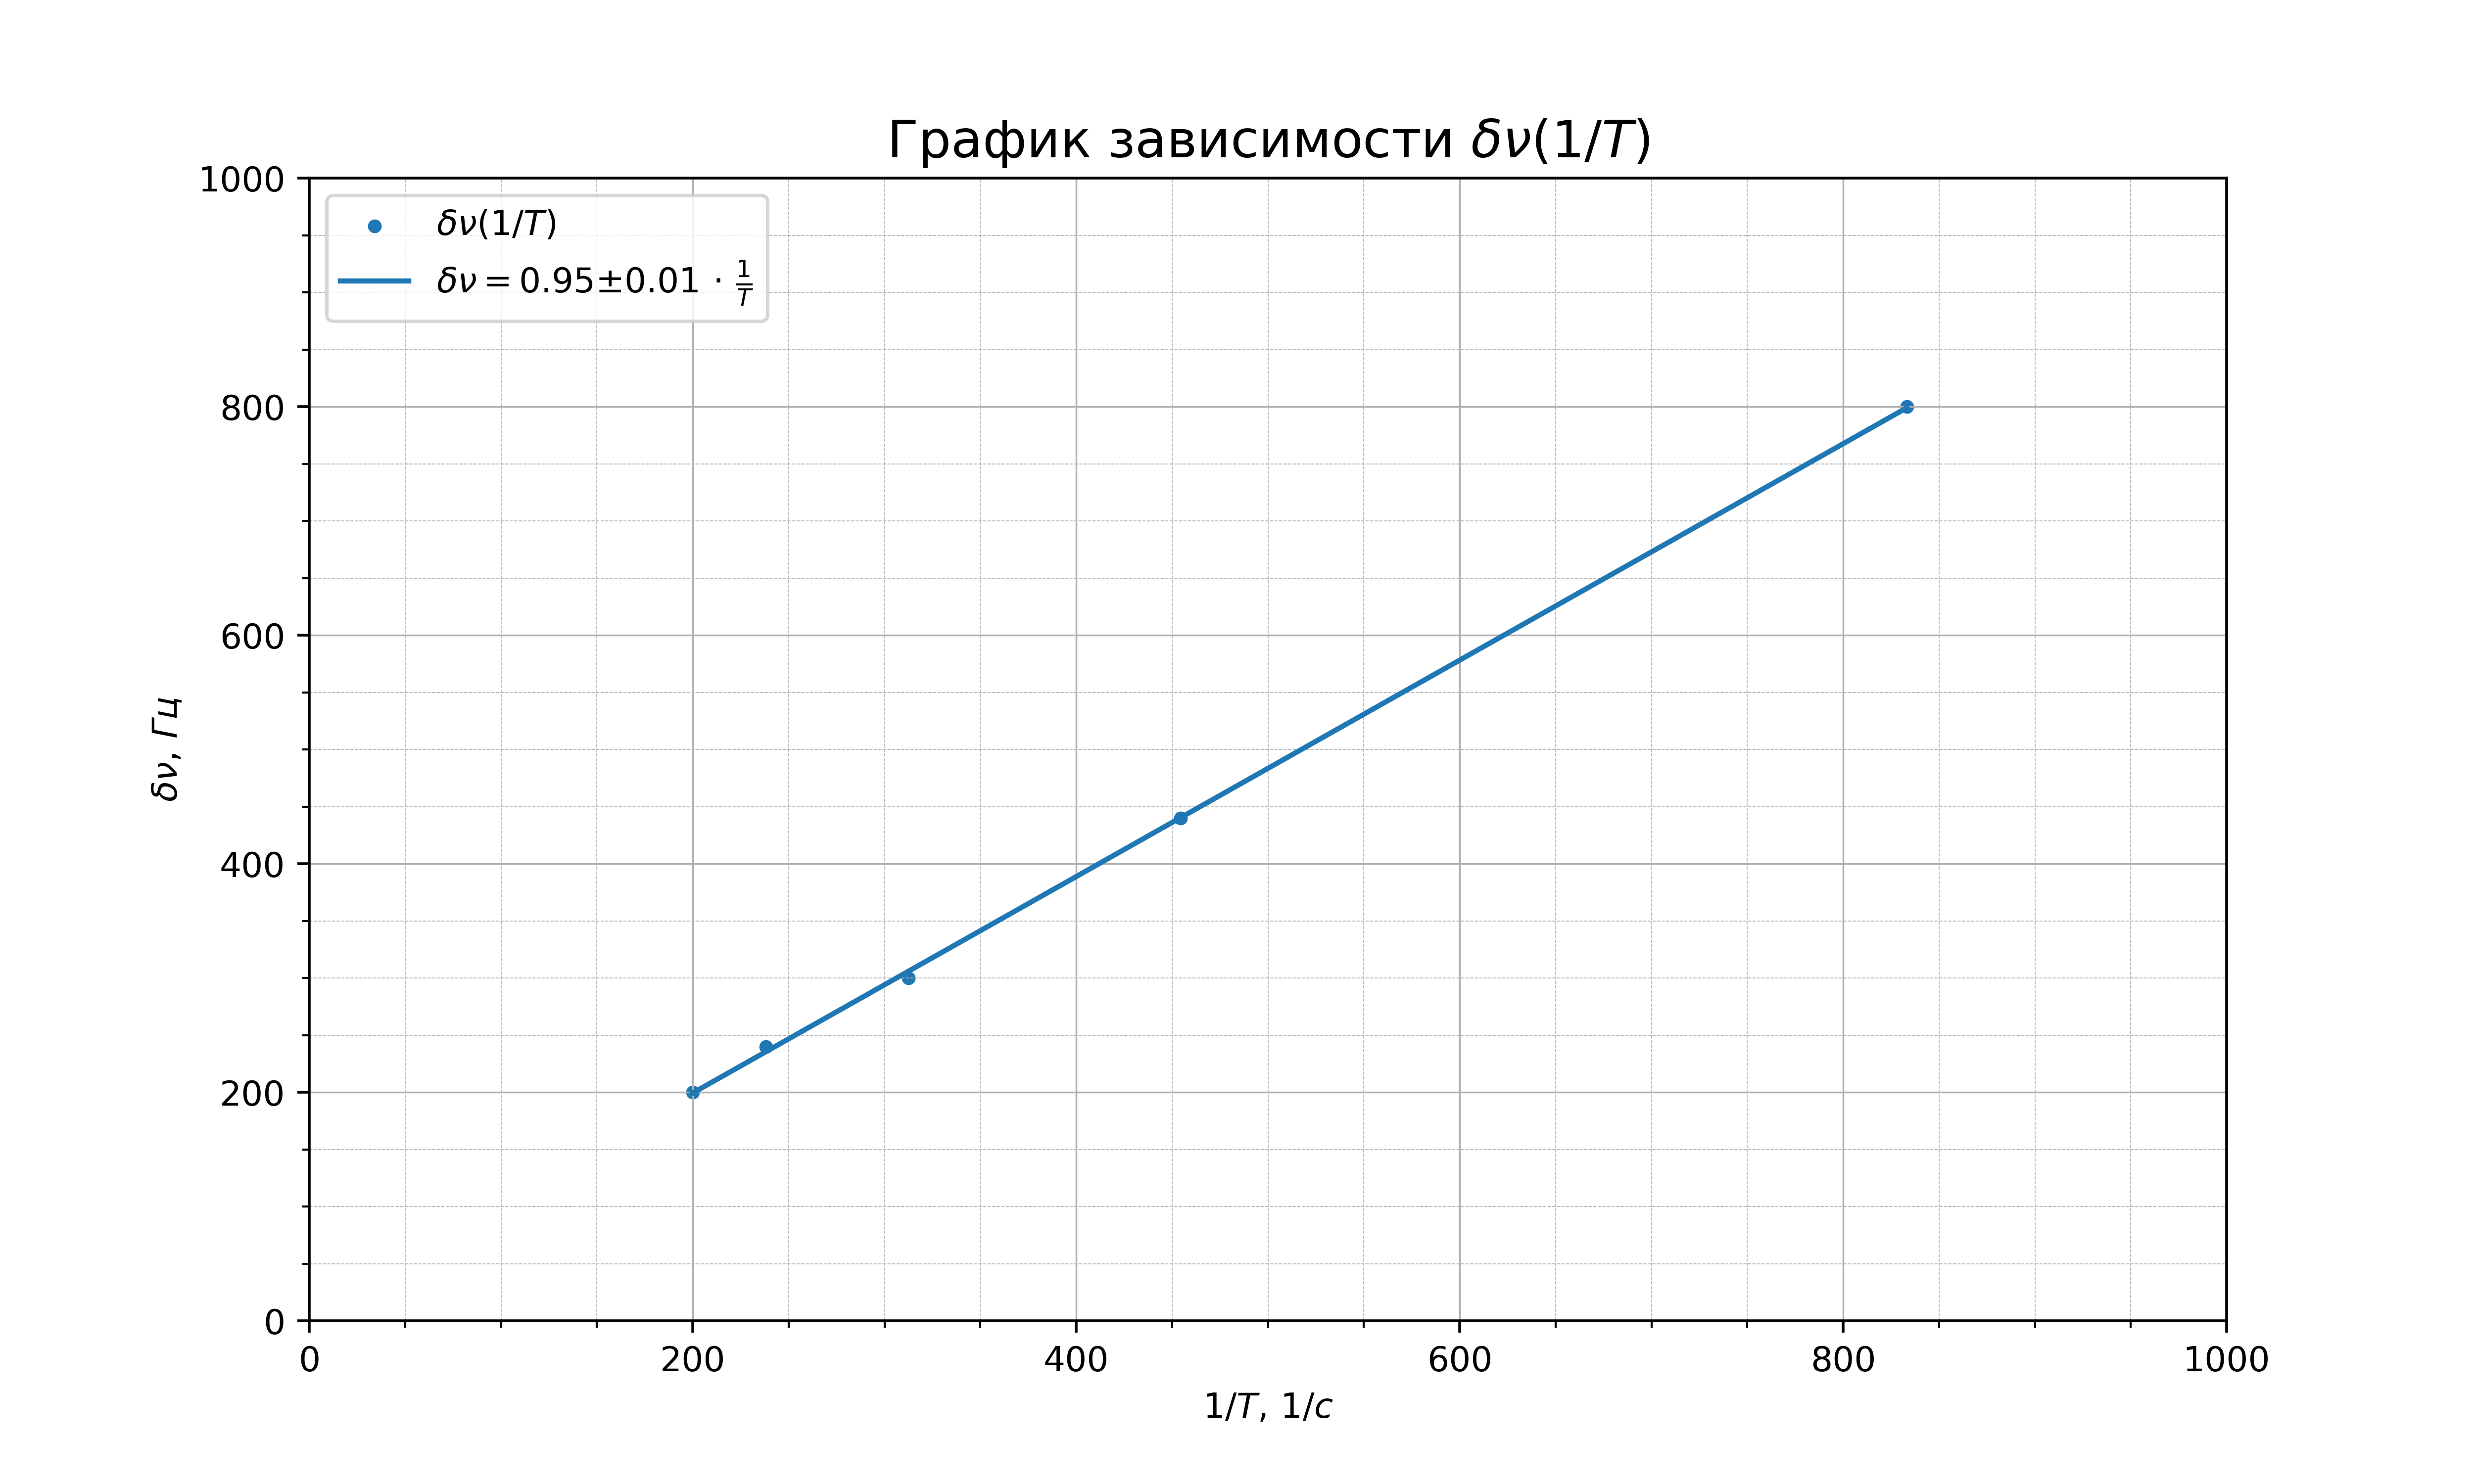
\includegraphics[scale=0.7]{3.6.1_2.png}
\end{flushleft}
\caption{График зависимости расстояния между соседними спектральными компонентами сигнала $\delta{\nu}$ от обратной величины периода повторения $1/T$}
\label{plot2}
\end{figure}

\newpage

\subsection{Исследование спектра амплитудно-модулированного сигнала}

Картина сигнала представлена на рис.~\ref{ris20}. Измеренные значения: $A_{max} = 1,62~B$, $A_{min} = 0,56~B$, $m = \frac{A_{max} - A_{min}}{A_{max} + A_{min}} = 0,49 \approx 0,5$, а значит равенство справедливо. Спектры сигналов при различных $\nu_0$ и $\nu_{мод}$ представлены на рис.~\ref{ris21}-\ref{ris23}.

При фиксированных параметрах $\nu_0 = 60~кГц$ и $\nu_{мод} = 5~кГц$ была измерена зависимость отношения $a_{бок}/a_{осн}$ амплитуд боковой и основной спектральных линий от глубины модуляции $m$  в диапазоне от 10\% до 100\%. Измеренные значения представлены в таб.~\ref{tab4}.

\begin{table}[h!]
\begin{center}
\begin{tabular}{|c|c|c|c|c|c|c|}
\hline
$m$ & $a_{бок}, мВ$ & $\delta_{a_{бок}}, мВ$ & $a_{осн}, мВ$ & $\delta_{a_{осн}}, мВ$ & $a_{бок}/a_{осн}$ & $\delta_{a_{бок}/a_{осн}}$ \\ \hline
0,1 & 32 & 2 & 728 & 2 & 0,044 & 0,003 \\ \hline
0,3 & 104 & 2 & 728 & 2 & 0,143 & 0,003 \\ \hline
0,5 & 176 & 2 & 728 & 2 & 0,242 & 0,003 \\ \hline
0,7 & 256 & 2 & 728 & 2 & 0,352 & 0,003 \\ \hline
0,9 & 328 & 2 & 728 & 2 & 0,451 & 0,003 \\ \hline
1 & 364 & 2 & 728 & 2 & 0,500 & 0,003 \\ \hline
\end{tabular}
\end{center}
\caption{Результаты измерений зависимости $a_{бок}/a_{осн}$ от $m$}
\label{tab4}
\end{table}

Полученный график зависимости $a_{бок}/a_{осн}$ от $m$ представлен на рис.~\ref{plot3}.

\begin{figure}[h!]
\begin{flushleft}
    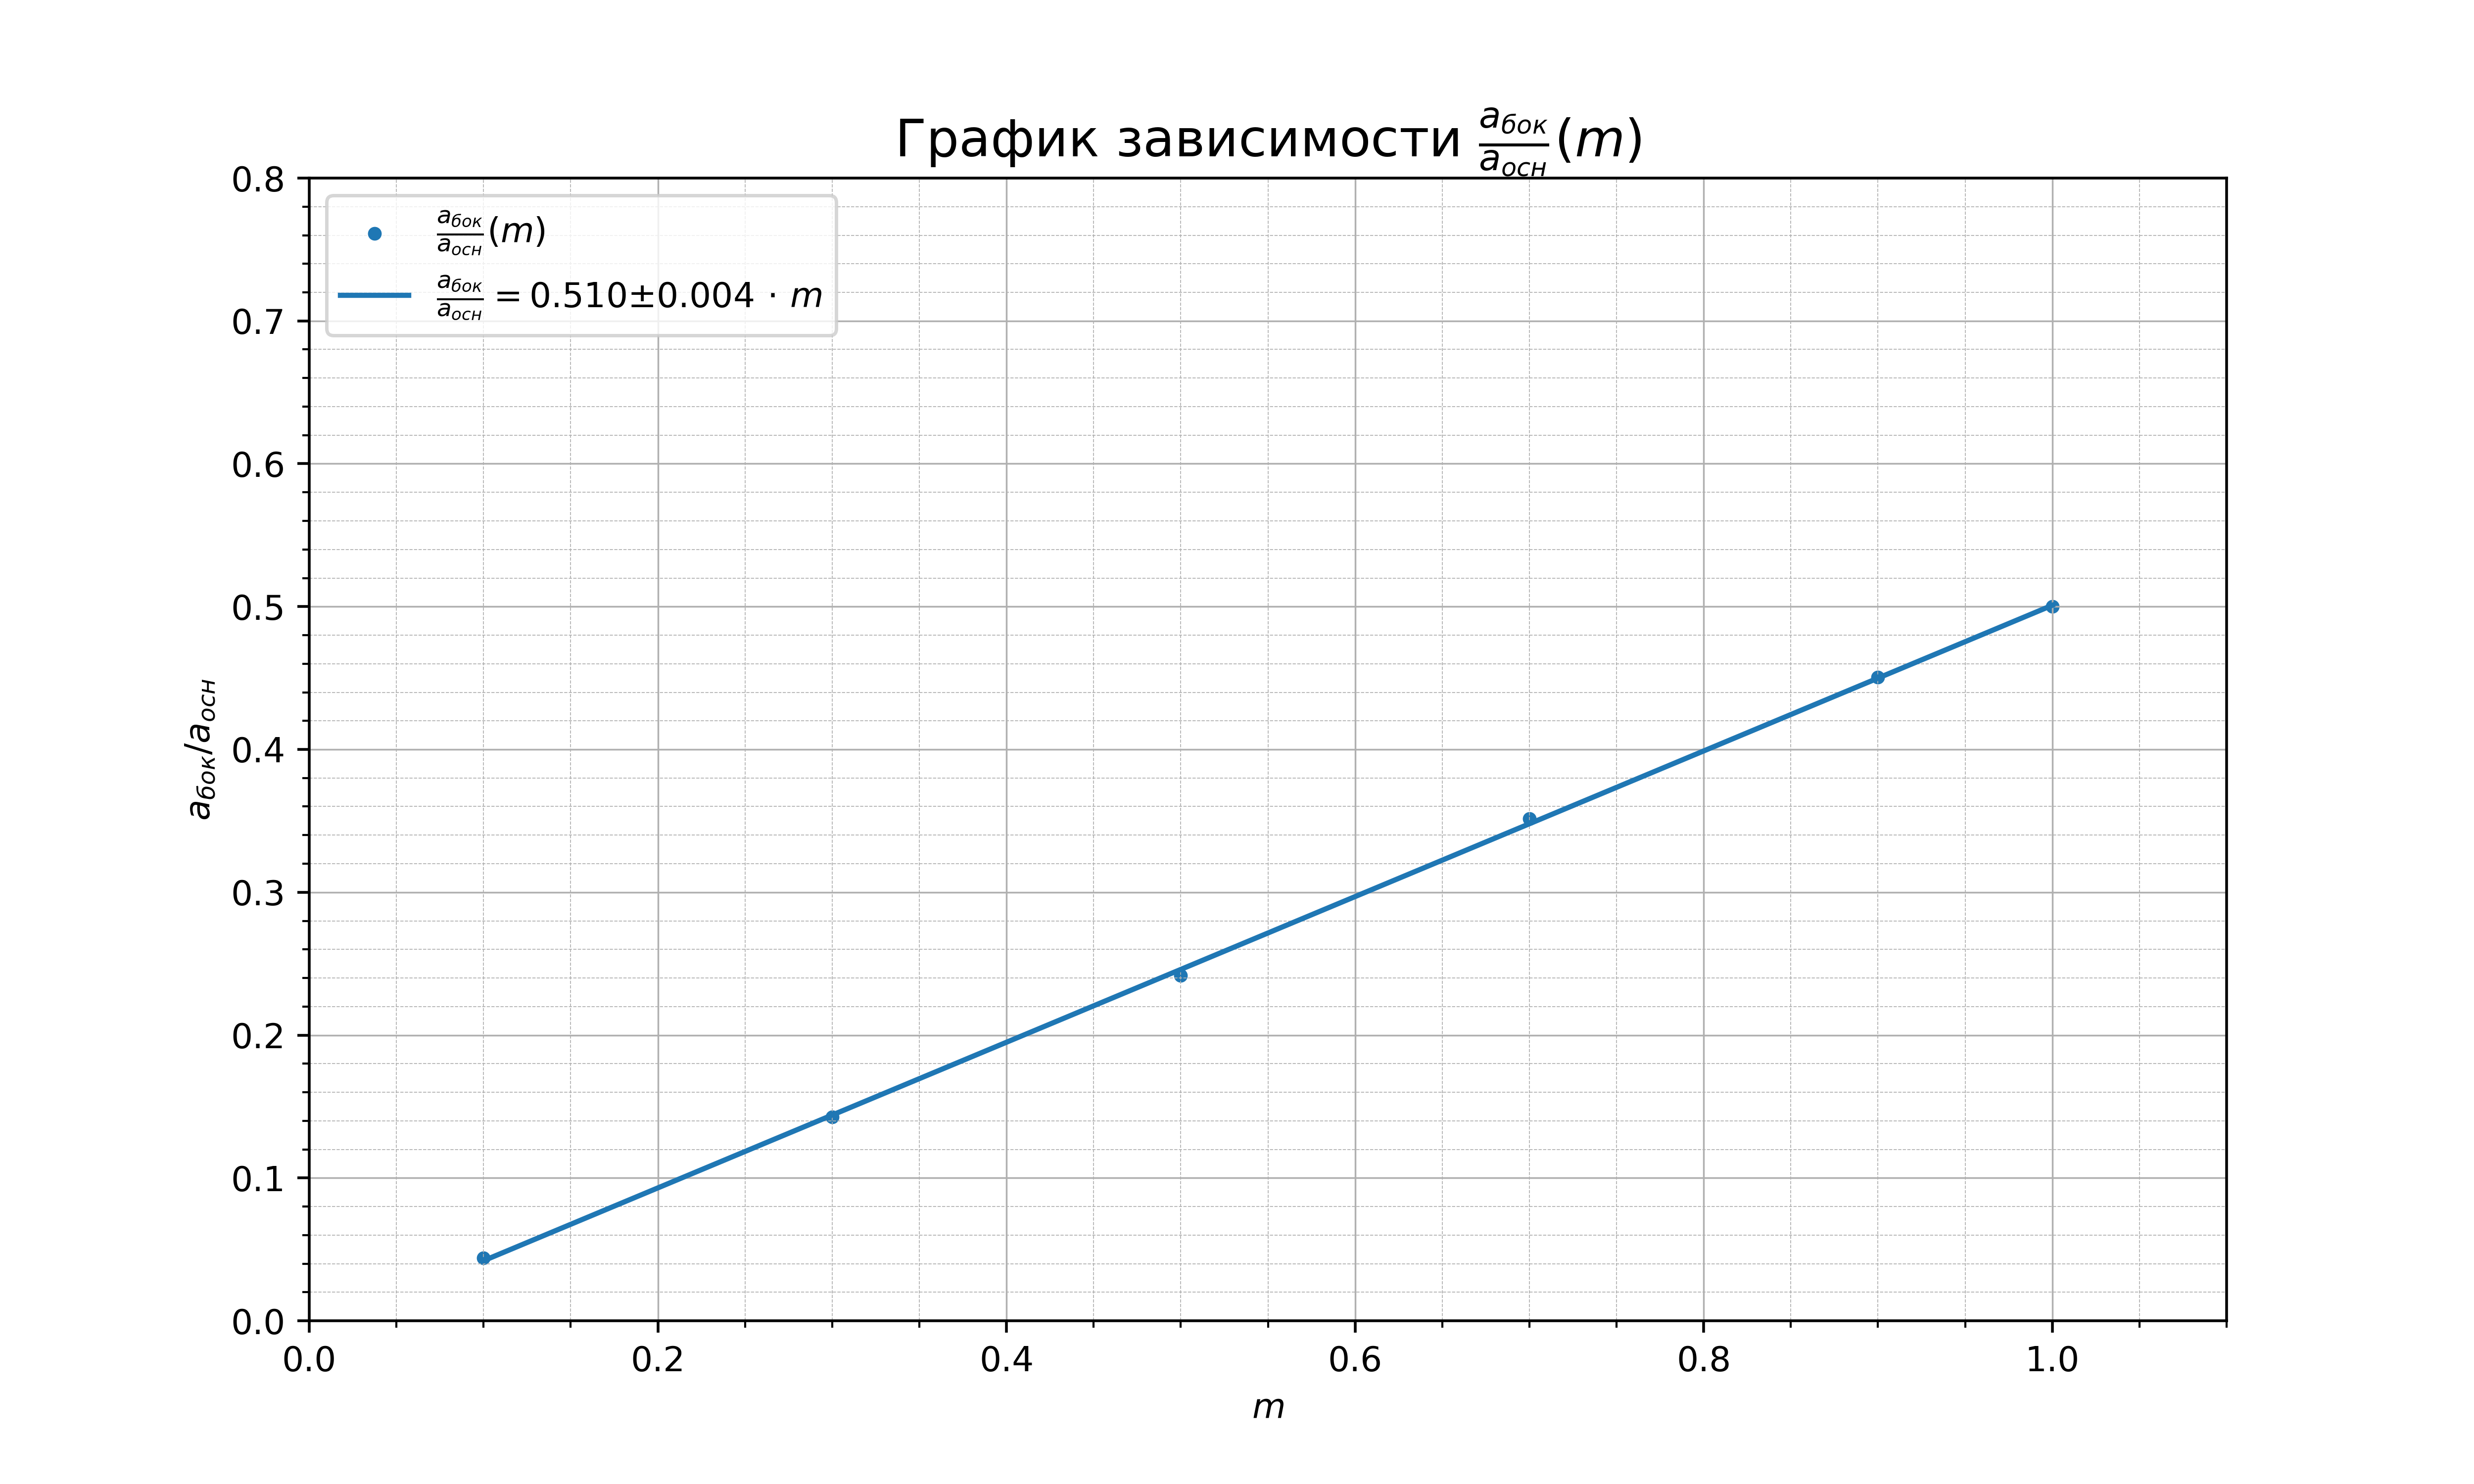
\includegraphics[scale=0.7]{3.6.1_3.png}
\end{flushleft}
\caption{График зависимости отношения $a_{бок}/a_{осн}$ амплитуд боковой и основной спектральных линий от глубины модуляции $m$}
\label{plot3}
\end{figure}

\newpage

\subsection{Исследование спектра сигнала, модулированного по фазе}

Спектры сигналов представлены на рис.~\ref{ris24}-\ref{ris25}.

\section{Обсуждение результатов и выводы}

В данной работе был исследован спектральный состав периодических электрических сигналов.

При исследовании спектра периодической последовательности прямоугольных импульсов при фиксированных параметрах $\nu_{повт}$ и $\tau$ были измерены амплитуды и частоты первых 6 гармоник (таб.~\ref{tab1}). Измеренные значения соответствуют рассчитанным теоретически. Также была измерена зависимость ширины спектра $\Delta{\nu}$ от времени импульса $\tau$. Из полученной зависимости (рис.~\ref{plot1}) следует: $$\Delta{\nu} \cdot \tau \backsimeq 1,01\pm0,01,$$ что соответствует соотношению неопределённостей в рамках погрешности. Основной вклад в погрешность вносит определение коэффициента зависимости, так как благодаря использованию цифровых приборов другие источники погрешности отсутствуют или их влияние несущественно.

При исследовании спектра периодической последовательности цугов была измерена зависимость расстояния $\delta{\nu}$ между соседними спектральными компонентами сигнала от периода $T$ повторения импульсов. Из полученной зависимости (рис.~\ref{plot2}) следует: $$\delta{\nu} \cdot \tau \backsimeq 0,95\pm0,01,$$ что близко к соотношению неопределённостей. Здесь основной вклад в погрешность также вносит определение коэффициента зависимости.

При исследовании спектра амплитудно-модулированного сигнала была измерена зависимость отношения $a_{бок}/a_{осн}$ амплитуд боковой и основной спектральных линий от глубины модуляции $m$. Из полученной зависимости (рис.~\ref{plot3}) следует: $$\frac{a_{бок}}{a_{осн}} = 0,510\pm0,004 \cdot m,$$ что соответствует теоретической зависимости $\frac{a_{бок}}{a_{осн}} = \frac{m}{2}$. Аналогично здесь основной вклад в погрешность вносит определение коэффициента зависимости.

Также в данной работе был изучен спектр сигнала, модулированного по фазе. Спектры сигналов при различном максимальном отклонении $\varphi_m$ приведены на рис.~\ref{ris24}-\ref{ris25}.

\section{Приложение}

\begin{figure}[h!]
\begin{flushleft}
    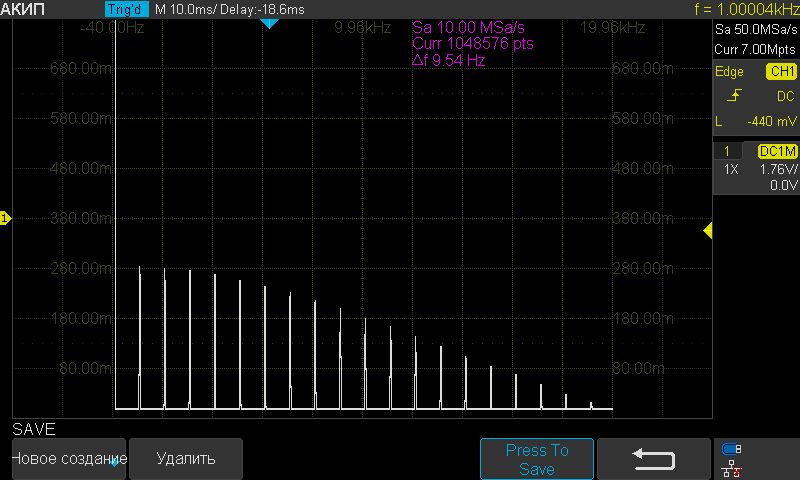
\includegraphics[scale=0.5]{AKIP0001.png}
\end{flushleft}
\caption{Спектр периодической последовательности прямоугольных импульсов при \newline $\nu_{повт} = 1~кГц$, $\tau = 50~мкс$}
\label{ris7}
\end{figure}

\begin{figure}[h!]
\begin{flushleft}
    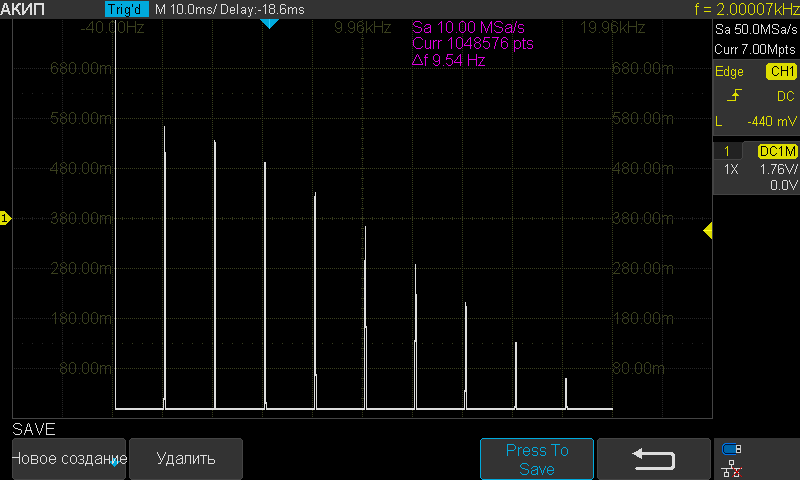
\includegraphics[scale=0.5]{AKIP0002.png}
\end{flushleft}
\caption{Спектр периодической последовательности прямоугольных импульсов при \newline $\nu_{повт} = 2~кГц$, $\tau = 50~мкс$}
\label{ris8}
\end{figure}

\begin{figure}[h!]
\begin{flushleft}
    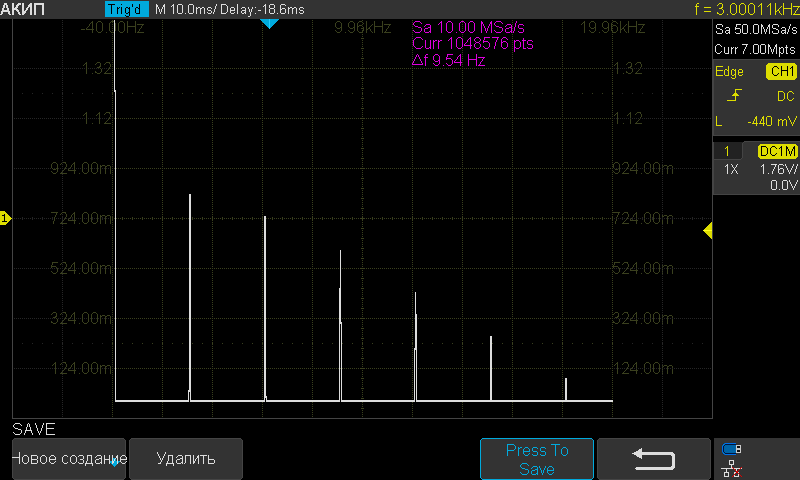
\includegraphics[scale=0.5]{AKIP0003.png}
\end{flushleft}
\caption{Спектр периодической последовательности прямоугольных импульсов при \newline $\nu_{повт} = 3~кГц$, $\tau = 50~мкс$}
\label{ris9}
\end{figure}

\begin{figure}[h!]
\begin{flushleft}
    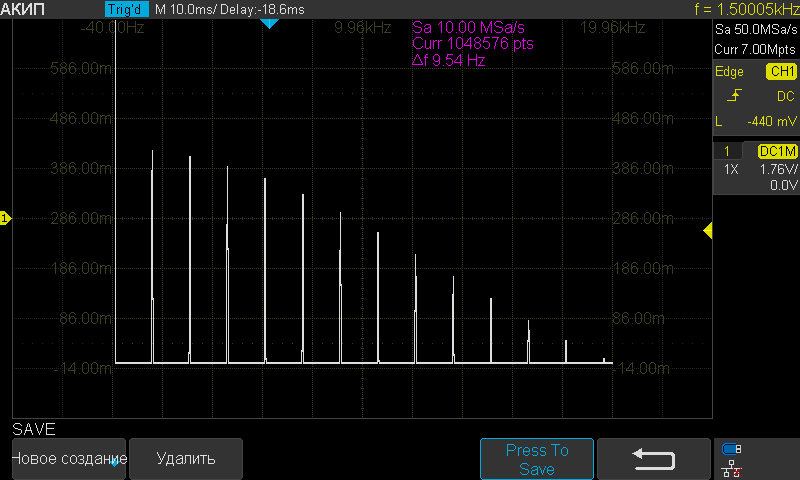
\includegraphics[scale=0.5]{AKIP0004.png}
\end{flushleft}
\caption{Спектр периодической последовательности прямоугольных импульсов при \newline $\nu_{повт} = 1,5~кГц$, $\tau = 50~мкс$}
\label{ris10}
\end{figure}

\begin{figure}[h!]
\begin{flushleft}
    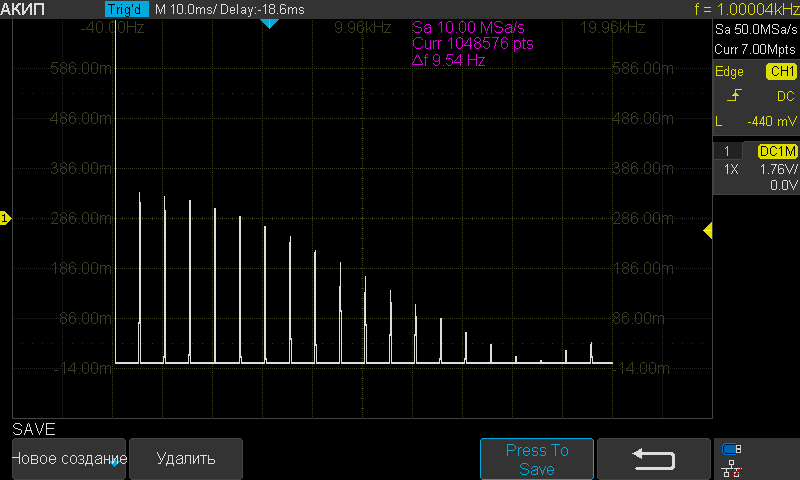
\includegraphics[scale=0.5]{AKIP0005.png}
\end{flushleft}
\caption{Спектр периодической последовательности прямоугольных импульсов при \newline $\nu_{повт} = 1~кГц$, $\tau = 60~мкс$}
\label{ris11}
\end{figure}

\begin{figure}[h!]
\begin{flushleft}
    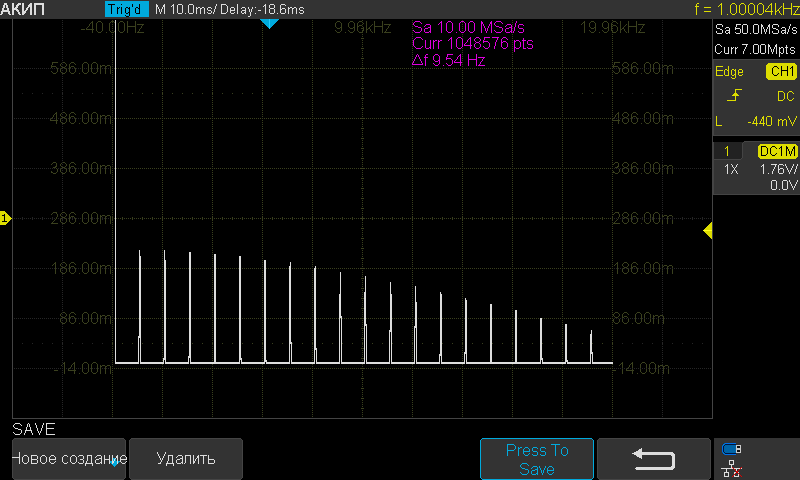
\includegraphics[scale=0.5]{AKIP0006.png}
\end{flushleft}
\caption{Спектр периодической последовательности прямоугольных импульсов при \newline $\nu_{повт} = 1~кГц$, $\tau = 40~мкс$}
\label{ris12}
\end{figure}

\begin{figure}[h!]
\begin{flushleft}
    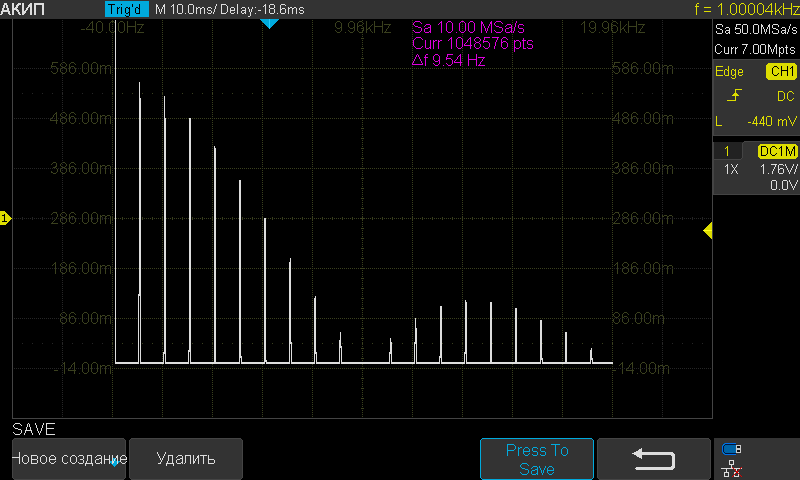
\includegraphics[scale=0.5]{AKIP0007.png}
\end{flushleft}
\caption{Спектр периодической последовательности прямоугольных импульсов при \newline $\nu_{повт} = 1~кГц$, $\tau = 100~мкс$}
\label{ris13}
\end{figure}

\begin{figure}[h!]
\begin{flushleft}
    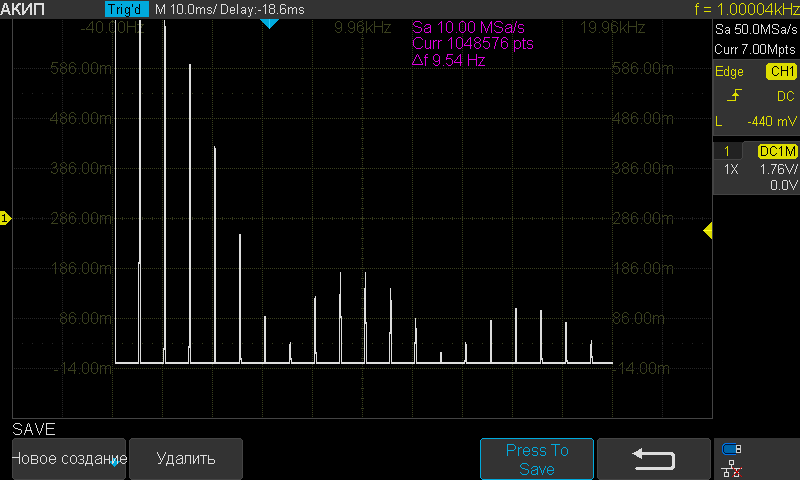
\includegraphics[scale=0.5]{AKIP0008.png}
\end{flushleft}
\caption{Спектр периодической последовательности прямоугольных импульсов при \newline $\nu_{повт} = 1~кГц$, $\tau = 150~мкс$}
\label{ris14}
\end{figure}

\begin{figure}[h!]
\begin{flushleft}
    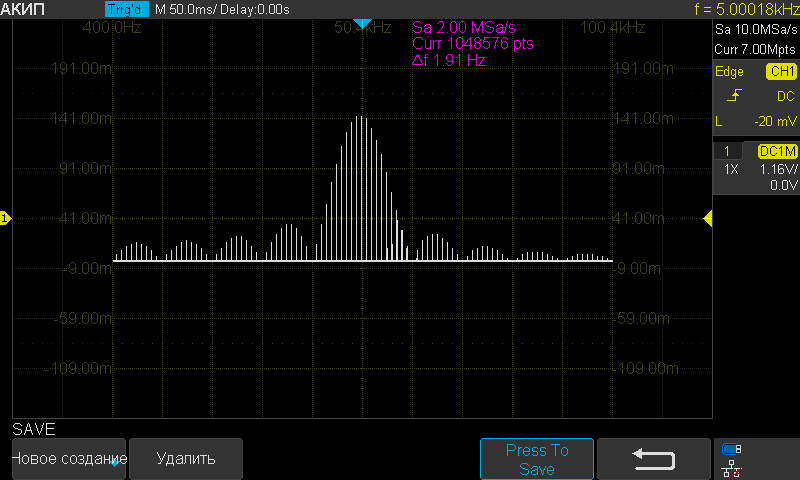
\includegraphics[scale=0.5]{AKIP0009.png}
\end{flushleft}
\caption{Спектр периодической последовательности цугов при $\nu_0 = 50~кГц$, $T = 1~мс$, $N = 5$}
\label{ris15}
\end{figure}

\begin{figure}[h!]
\begin{flushleft}
    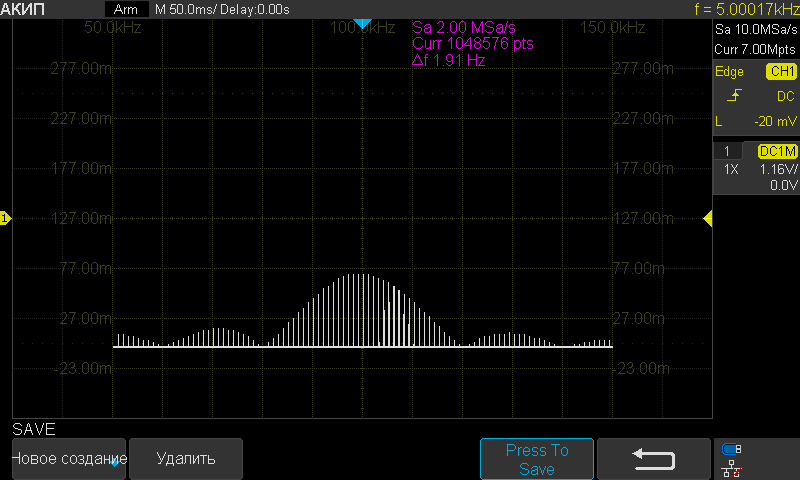
\includegraphics[scale=0.5]{AKIP0010.png}
\end{flushleft}
\caption{Спектр периодической последовательности цугов при $\nu_0 = 100~кГц$, $T = 1~мс$, $N = 5$}
\label{ris16}
\end{figure}

\begin{figure}[h!]
\begin{flushleft}
    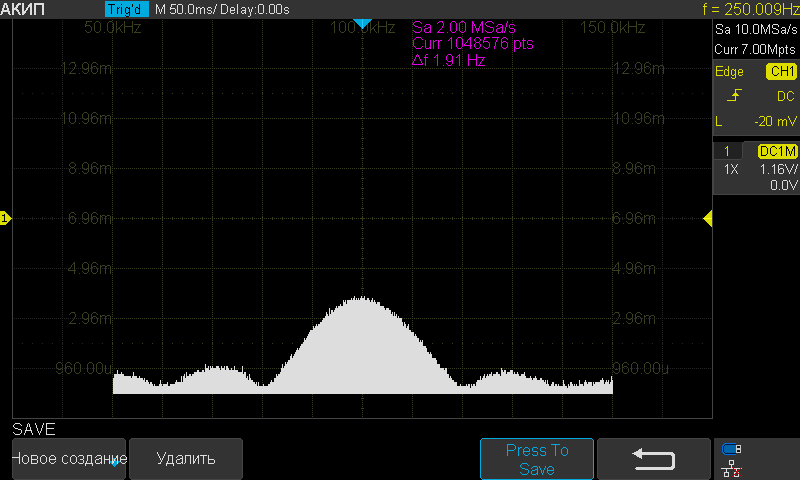
\includegraphics[scale=0.5]{AKIP0011.png}
\end{flushleft}
\caption{Спектр периодической последовательности цугов при $\nu_0 = 100~кГц$, $T = 20~мс$, $N = 5$}
\label{ris17}
\end{figure}

\begin{figure}[h!]
\begin{flushleft}
    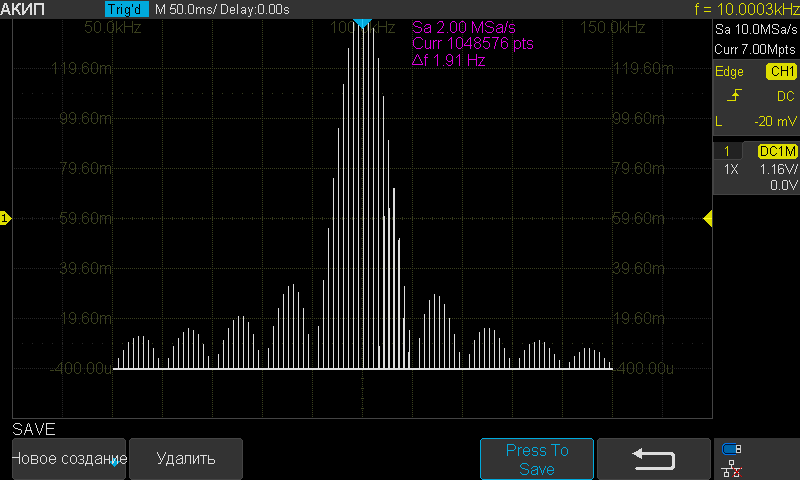
\includegraphics[scale=0.5]{AKIP0012.png}
\end{flushleft}
\caption{Спектр периодической последовательности цугов при $\nu_0 = 100~кГц$, $T = 1~мс$, $N = 10$}
\label{ris18}
\end{figure}

\begin{figure}[h!]
\begin{flushleft}
    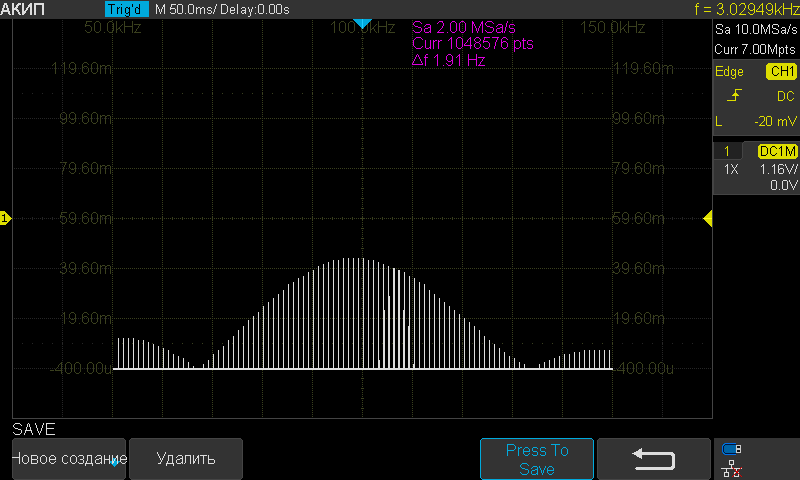
\includegraphics[scale=0.5]{AKIP0013.png}
\end{flushleft}
\caption{Спектр периодической последовательности цугов при $\nu_0 = 100~кГц$, $T = 1~мс$, $N = 3$}
\label{ris19}
\end{figure}

\begin{figure}[h!]
\begin{flushleft}
    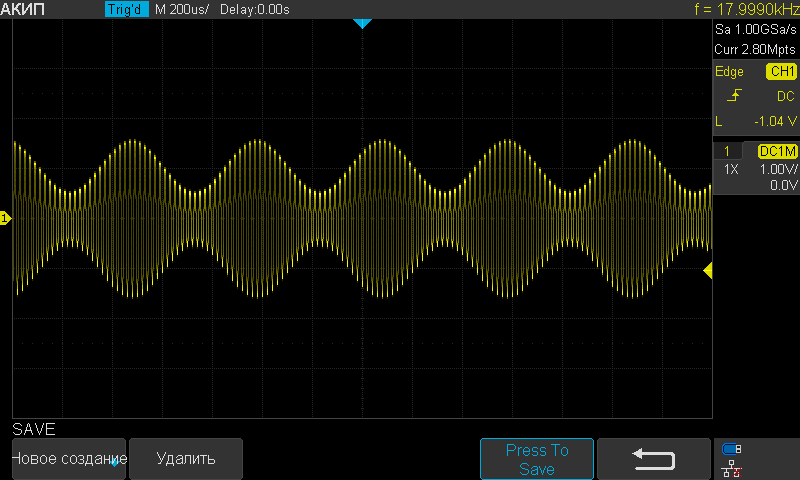
\includegraphics[scale=0.5]{AKIP0014.png}
\end{flushleft}
\caption{Амплитудно-модулированный сигнал при $\nu_0 = 50~кГц$, $\nu_{мод} = 2~кГц$ и $m = 0,5$}
\label{ris20}
\end{figure}

\begin{figure}[h!]
\begin{flushleft}
    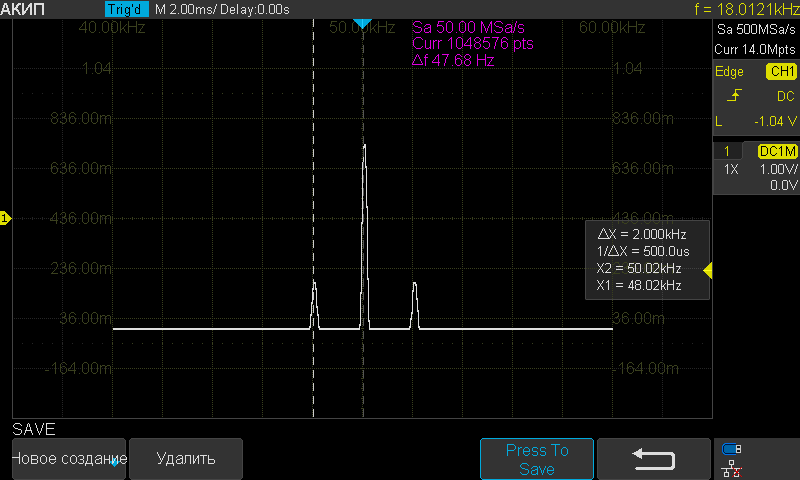
\includegraphics[scale=0.5]{AKIP0015.png}
\end{flushleft}
\caption{Спектр амплитудно-модулированного сигнала при $\nu_0 = 50~кГц$, $\nu_{мод} = 2~кГц$ и $m = 0,5$}
\label{ris21}
\end{figure}

\begin{figure}[h!]
\begin{flushleft}
    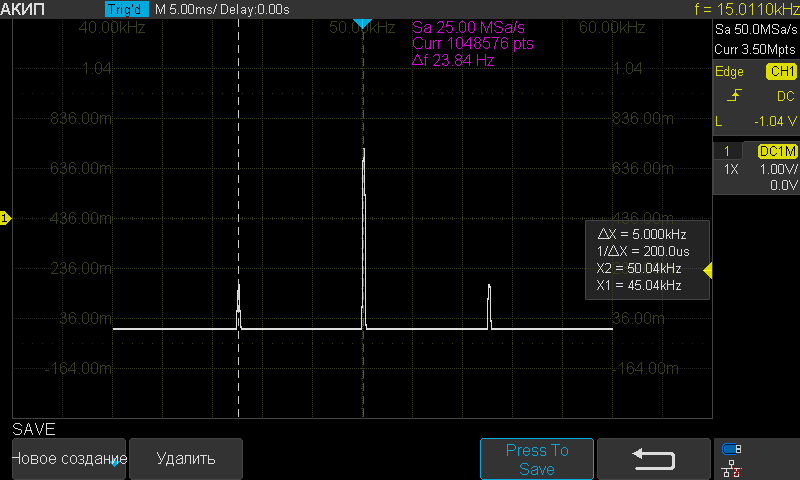
\includegraphics[scale=0.5]{AKIP0016.png}
\end{flushleft}
\caption{Спектр амплитудно-модулированного сигнала при $\nu_0 = 50~кГц$, $\nu_{мод} = 5~кГц$ и $m = 0,5$}
\label{ris22}
\end{figure}

\begin{figure}[h!]
\begin{flushleft}
    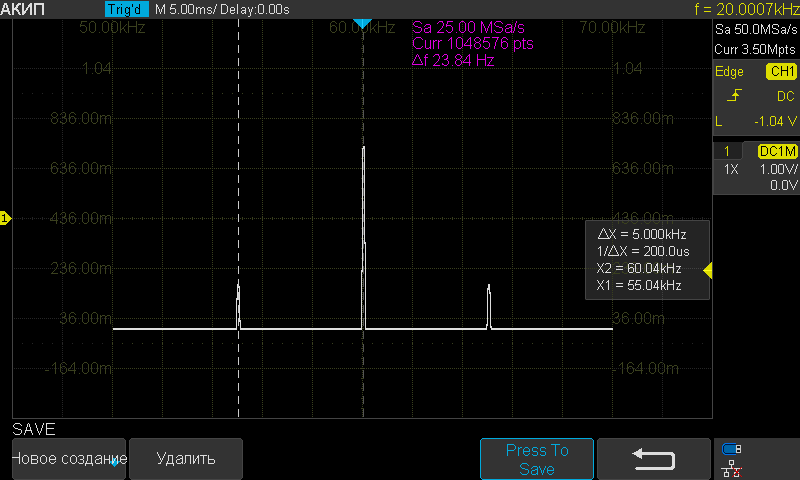
\includegraphics[scale=0.5]{AKIP0017.png}
\end{flushleft}
\caption{Спектр амплитудно-модулированного сигнала при $\nu_0 = 60~кГц$, $\nu_{мод} = 5~кГц$ и $m = 0,5$}
\label{ris23}
\end{figure}

\begin{figure}[h!]
\begin{flushleft}
    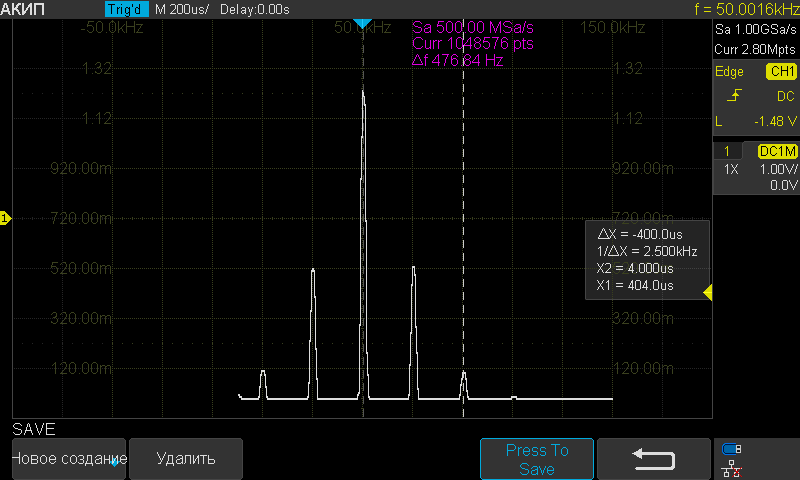
\includegraphics[scale=0.5]{AKIP0018.png}
\end{flushleft}
\caption{Спектр модулированного по фазе сигнала при $\nu_0 = 50~кГц$, $\nu_{мод} = 2~кГц$ и $\varphi_m = 10^{\circ}$}
\label{ris24}
\end{figure}

\begin{figure}[h!]
\begin{flushleft}
    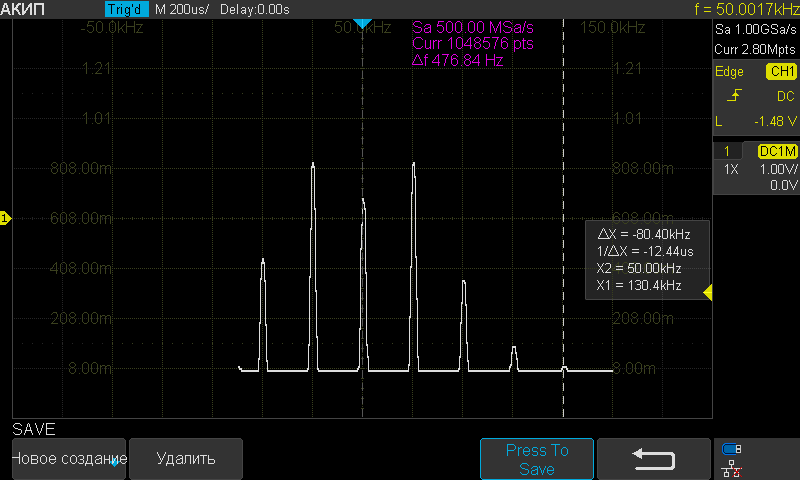
\includegraphics[scale=0.5]{AKIP0019.png}
\end{flushleft}
\caption{Спектр модулированного по фазе сигнала при $\nu_0 = 50~кГц$, $\nu_{мод} = 2~кГц$ и $\varphi_m = 90^{\circ}$}
\label{ris25}
\end{figure}

\end{document}
